\documentclass[aspectratio=1610,t]{beamer}

\usepackage[english]{babel}
\usepackage{hyperref}
\usepackage{minted}
\usepackage{alltt}
\usepackage{amsmath}
\usepackage{graphicx}
\usepackage{xcolor}
\usepackage[utf8]{inputenc}
\usepackage[T1]{fontenc}

\usetheme{metropolis}
\usemintedstyle{xcode}
\definecolor{codebg}{RGB}{247, 247, 246}
\setbeamercolor{background canvas}{bg=white}
\hypersetup{colorlinks,linkcolor=,urlcolor=orange}

\title{Lecture 6: Cargo and Modules}
\date{March 14, 2023}
\author{Barinov Denis}
\institute{barinov.diu@gmail.com}

\begin{document}

% ----------------------------------------------------------------- %

\begin{frame}
\maketitle
\end{frame}

% ----------------------------------------------------------------- %

\begin{frame}[c]
\centering\Huge\textbf{Cargo and Modules}
\end{frame}

% ----------------------------------------------------------------- %

\begin{frame}[fragile]
\frametitle{Cargo}
Cargo is the Rust language package manager. It's one of the greatest things about Rust!

What Cargo does do?

\begin{itemize}
    \item Downloads and manages your dependencies.
    \item Compiles your packages.
    \item Makes distributable packages.
    \item And more!
\end{itemize}
\end{frame}

% ----------------------------------------------------------------- %

\begin{frame}[fragile]
\frametitle{Crate}
A crate is a compilation unit in Rust. It's like a package in other languages. An example of crate created by \texttt{cargo new --bin example} command:

\begin{verbatim}
    example
    ├── Cargo.lock
    ├── Cargo.toml
    └── src
    └── main.rs
\end{verbatim}

Packages can be uploaded to \href{https://crates.io}{crates.io}, the Rust community's crate registry. It makes them available to everyone, and users will have an opportunity to use your crate as a dependency at the manifest.
\end{frame}

% ----------------------------------------------------------------- %

\begin{frame}[fragile]
\frametitle{Crate}
A package is described using manifest file called \texttt{Cargo.toml}. Here's an example:

\begin{minted}{toml}
    [package]
    name = "example"
    version = "0.1.0"
    edition = "2021"

    [dependencies]
    clap = "3.1.0"
\end{minted}
\end{frame}

% ----------------------------------------------------------------- %

\begin{frame}[fragile]
\frametitle{Crate: \texttt{Cargo.toml}}
\texttt{Cargo.toml} consists of multiple entries.\footnote{\href{https://doc.rust-lang.org/cargo/reference/manifest.html#the-rust-version-field}{The Manifest Format}} Here's an example:

\begin{itemize}
    \item \texttt{[package]} has the meta information about package like name, version, authors, edition, compiler version, build scripts...
    \item \texttt{[dependencies]} describes dependencies of our package, their versions, needed features.
    \item \texttt{[features]} provides a mechanism to express conditional compilation and optional dependencies.
    \item And more!
\end{itemize}
\end{frame}

% ----------------------------------------------------------------- %

\begin{frame}[fragile]
\frametitle{Crate}
There are multiple types of crates.\footnote{\href{https://doc.rust-lang.org/reference/linkage.html}{Linkage, The Rust Reference}}

\begin{itemize}
    \item \texttt{bin} - a runnable executable. It's default crate type
    \item \texttt{lib} - a ``compiler recommended'' Rust library.
    \item \texttt{dylib} - a dynamic Rust library.
    \item \texttt{staticlib} - a static system library.
    \item \texttt{cdylib} - a C dynamic library.
    \item \texttt{rlib} - a ``Rust library'' file.
    \item \texttt{proc-macro} - a procedural macros crate.
\end{itemize}

\texttt{bin} or \texttt{lib} types should be sufficient for all compilation needs.
\end{frame}

% ----------------------------------------------------------------- %

\begin{frame}[fragile]
\frametitle{Crate: versions}
In Cargo, versions of packages \textbf{must be changed} accordingly to Semantic Versioning (semver).\footnote{\href{https://semver.org}{Semantic Versioning 2.0.0}}

Given a version number \texttt{MAJOR.MINOR.PATCH}, increment the:

\begin{itemize}
    \item \texttt{MAJOR} version when you make incompatible API changes.
    \item \texttt{MINOR} version when you add functionality in a backwards compatible manner.
    \item \texttt{PATCH} version when you make backwards compatible bug fixes.
\end{itemize}
\end{frame}

% ----------------------------------------------------------------- %

\begin{frame}[fragile]
\frametitle{Crate: versions}
For instance, this version changes are legal:\footnote{\href{https://doc.rust-lang.org/cargo/reference/semver.html}{SemVer Compatibility}}

\begin{itemize}
    \item \texttt{1.3.7} -> \texttt{1.3.8} (bug fix).
    \item \texttt{1.5.5} -> \texttt{1.6.0} (added functionality).
    \item \texttt{1.7.2} -> \texttt{2.0.0} (major update, incompatible changes).
\end{itemize}

If your \texttt{MAJOR} version number is 0, Cargo will treat \texttt{MINOR} as \texttt{MAJOR} and \texttt{PATCH} as \texttt{MINOR}.
\end{frame}

% ----------------------------------------------------------------- %

\begin{frame}[fragile]
\frametitle{Crate: versions}
In \texttt{Cargo.toml}:

\begin{itemize}
    \item \texttt{\^{}1.2.3} - semver compatible (\texttt{< 2.0.0})
    \item \texttt{\~1.2.3} - only the last number is updated (\texttt{< 1.3.0})
    \item \texttt{1.2.*}
    \item \texttt{>= 1.2}
\end{itemize}

If your \texttt{MAJOR} version number is 0, Cargo will treat \texttt{MINOR} as \texttt{MAJOR} and \texttt{PATCH} as \texttt{MINOR}.
\end{frame}

% ----------------------------------------------------------------- %

\begin{frame}[fragile]
\frametitle{\texttt{Cargo.toml} vs \texttt{Cargo.lock}}
\begin{itemize}
    \item \texttt{Cargo.toml} is about describing your dependencies in a broad sense, and is written by you.
    \item \texttt{Cargo.lock} contains exact information about your dependencies. It is maintained by Cargo and should not be manually edited.
\end{itemize}

\visible<2->{
    The purpose of a \texttt{Cargo.lock} lockfile is to describe the state of the world at the time of a successful build.
}

\visible<3->{
    This property is the most desirable for packages that are at the very end of the dependency chain (binaries).
}

\visible<4->{
    But the library is not only used by the library developers, but also any downstream consumers of the library. Libraries specify semver requirements for their dependencies but cannot see the full picture. Only end products like binaries have a full picture to decide what versions of dependencies should be used.
}
\end{frame}

% ----------------------------------------------------------------- %

\begin{frame}[fragile]
\frametitle{Rust versions}
Rust version changes accordingly to semver, but how this exactly works?

\begin{itemize}
    \item<1-> Before version 1.0, as a new product, Rust changed frequently and hadn't given any guarantees about how your code will be compiled in future releases.
    \item<2-> After the release of 1.0, Rust started following one of the variations of ``stability without stagnation'' model, first introduced in web browsers.
    \item<3-> New work lands directly in the master branch.
    \item<4-> Each day, the last successful build from the master becomes the new nightly release.
    \item<5-> Every six weeks, a beta branch is created from the current state of the master, and the previous beta is promoted to be the new stable release.
\end{itemize}
\end{frame}

% ----------------------------------------------------------------- %

\begin{frame}[fragile]
\frametitle{Rust versions}
Rust version changes accordingly to semver, but how this exactly works?

\begin{itemize}
    \item<1-> In short, there are three release channels - nightly, beta, and stable - with regular, frequent promotions from one channel to the next.
    \item<2-> New features and new APIs will be flagged as unstable via feature gates and stability attributes respectively. Unstable features and standard library APIs will only be available on the nightly branch, and only if you explicitly ``opt-in'' to the instability.
    \item<3-> But sometimes, make small changes to the language that are not backward compatible. The most obvious example is introducing a new keyword, which would invalidate variables with the same name.
    \item<4-> For instance, before 2018 there were no \texttt{async} and \texttt{await} keywords.
    \item<5-> When the release is about to break code, it becomes a part of the new edition. The choice of edition is made in \texttt{Cargo.toml} for a crate.
\end{itemize}
\end{frame}

% ----------------------------------------------------------------- %

\begin{frame}[fragile]
\frametitle{Rust versions}
Rust version changes accordingly to semver, but how this exactly works?

\begin{itemize}
    \item<1-> This ensures that the decision to migrate to a newer edition is a ``private one'' that the crate can make without affecting your downstream crates.
    \item<2-> To automate migration, there's \texttt{cargo fix --edition} command.
    \item<3-> For example, when migrating to Rust 2018, it changes anything named async to use the equivalent raw identifier syntax: \texttt{r\#async}.
\end{itemize}
\end{frame}

% ----------------------------------------------------------------- %

\begin{frame}[fragile]
\frametitle{\texttt{rustc}}
As you can see, we don't need to even know something about \texttt{rustc}! (expect version, of course)

This is one of the cool things about Cargo.

A detailed discussion of it is not part of this lecture.
\end{frame}

% ----------------------------------------------------------------- %

\begin{frame}[c]
\centering\Huge\textbf{Modules}
\end{frame}

% ----------------------------------------------------------------- %

\begin{frame}[fragile]
\frametitle{Modules}
\begin{minted}[fontsize=\small]{rust}
    mod one {
        mod nested {
            mod nested2 {
                struct Foo { /* ... */ }
            }
            enum Count { /* ... */ }
        }
        trait MyTrait { /* ... */ }
    }
    mod two {
        struct Bar { /* ... */ }
        fn use_me() { /* ... */ }
    }
\end{minted}

\texttt{mod} keyword defines a module. Modules are used to control the visibility of declarations inside it and to prevent namespace pollution.
\end{frame}

% ----------------------------------------------------------------- %

\begin{frame}[fragile]
\frametitle{Modules}
We can use the \texttt{use\_me} using full path:

\begin{minted}{rust}
    two::use_me();
\end{minted}
\end{frame}

% ----------------------------------------------------------------- %

\begin{frame}[fragile]
\frametitle{Modules}
We can use the \texttt{use\_me} using full path:

\begin{minted}{rust}
    two::use_me();
\end{minted}

This code won't compile:

\begin{minted}{rust}
error[E0603]: function `use_me` is private
  --> src/main.rs:16:12
   |
16 | two::use_me();
   |      ^^^^^^ private function
\end{minted}
\end{frame}

% ----------------------------------------------------------------- %

\begin{frame}[fragile]
\frametitle{Modules}
\begin{minted}[fontsize=\small]{rust}
    mod one {
        mod nested {
            mod nested2 {
                struct Foo { /* ... */ }
            }
            enum Count { /* ... */ }
        }
        trait MyTrait { /* ... */ }
    }
    mod two {
        struct Bar { /* ... */ }
        pub fn use_me() { /* ... */ }
    }
\end{minted}

We'll use \texttt{pub} keyword. It means ``make it private for all parent modules''.
\end{frame}

% ----------------------------------------------------------------- %

\begin{frame}[fragile]
\frametitle{Modules}
Next, we'll create \texttt{Foo} structure:

\begin{minted}{rust}
    let _ = one::nested::nested2::Foo {};
\end{minted}
\end{frame}

% ----------------------------------------------------------------- %

\begin{frame}[fragile]
\frametitle{Modules}
Next, we'll create \texttt{Foo} structure:

\begin{minted}{rust}
    let _ = one::nested::nested2::Foo {};
\end{minted}

We'll find out our module is private!

\begin{minted}{rust}
error[E0603]: module `nested` is private
  --> src/main.rs:16:18
   |
16 | let _ = one::nested::nested2::Foo {};
   |              ^^^^^^ private module
\end{minted}
\end{frame}

% ----------------------------------------------------------------- %

\begin{frame}[fragile]
\frametitle{Modules}
Rust modules are private by default!

But why compiler asked to make public the declaration of \texttt{nested}? And in the previous case - \texttt{two}?

\visible<2->{
    Because \texttt{one} and \texttt{two} are the part of our current module called \textbf{the root module}. We don't need to have rights to use the declarations in our current module - everything is public for us.
}

\visible<3->{
    Let's make \texttt{nested} public. Then we'll get compiler errors since \texttt{nested2} and \texttt{Foo} are private and make them public them too.
}
\end{frame}

% ----------------------------------------------------------------- %

\begin{frame}[fragile]
\frametitle{Modules}
\begin{minted}[fontsize=\small]{rust}
    mod one {
        pub mod nested {
            pub mod nested2 {
                pub struct Foo { /* ... */ }
            }
            enum Count { /* ... */ }
        }
        trait MyTrait { /* ... */ }
    }
    mod two {
        struct Bar { /* ... */ }
        pub fn use_me() { /* ... */ }
    }
\end{minted}
\end{frame}

% ----------------------------------------------------------------- %

\begin{frame}[fragile]
\frametitle{Modules}
\begin{minted}[fontsize=\small]{rust}
    mod one {
        pub mod nested {
            mod nested2 { // No 'pub'
                pub struct Foo { /* ... */ }
            }
            enum Count { /* ... */ }
        }
        trait MyTrait { /* ... */ }
    }
    mod two {
        struct Bar { /* ... */ }
        pub fn use_me() { /* ... */ }
    }
\end{minted}

Note that the following code won't make \texttt{Foo} available since \texttt{nested2} is private for us.
\end{frame}

% ----------------------------------------------------------------- %

\begin{frame}[fragile]
\frametitle{Modules}
\begin{minted}[fontsize=\small]{rust}
    mod one {
        pub mod nested {
            pub mod nested2 {
                pub struct Foo { bar: two::Bar }
            }
            enum Count { /* ... */ }
        }
        trait MyTrait { /* ... */ }
    }
    mod two {
        struct Bar { /* ... */ }
        pub fn use_me() { /* ... */ }
    }
\end{minted}

Next, we'll try to add a field \texttt{bar} of type \texttt{two::Bar} to \texttt{one::nested::nested2::Foo}.
\end{frame}

% ----------------------------------------------------------------- %

\begin{frame}[fragile]
\frametitle{Modules}
\begin{minted}[fontsize=\small]{rust}
error[E0433]: failed to resolve: use of undeclared crate
              or module `two`
  --> src/main.rs:4:35
   |
 4 | pub struct Foo { bar: two::Bar }
   |                       ^^^ use of undeclared crate or module `two`
\end{minted}

Why did this happen?

\visible<2->{
    By default, paths are relative. To make them absolute, we should use \texttt{crate} keyword (remember the path \texttt{/} in Unix systems?). In this case, our path will always start from the root module, not from the current module.
}
\end{frame}

% ----------------------------------------------------------------- %

\begin{frame}[fragile]
\frametitle{Modules}
\begin{minted}[fontsize=\small]{rust}
    mod one {
        pub mod nested {
            pub mod nested2 {
                pub struct Foo { bar: crate::two::Bar }
            }
            enum Count { /* ... */ }
        }
        trait MyTrait { /* ... */ }
    }
    mod two {
        // Note the 'pub'
        pub struct Bar { /* ... */ }
        pub fn use_me() { /* ... */ }
    }
\end{minted}

Since \texttt{Bar} is private in module \texttt{two}, we should use \texttt{pub} here too.
\end{frame}

% ----------------------------------------------------------------- %

\begin{frame}[fragile]
\frametitle{Modules}
Note that now we cannot construct \texttt{Foo} because it's \texttt{bar} field is private!

\begin{minted}{rust}
    let _ = one::nested::nested2::Foo { bar: two::Bar {} };
\end{minted}

\begin{minted}[fontsize=\small]{rust}
error[E0451]: field `bar` of struct `Foo` is private
  --> src/main.rs:17:41
   |
17 |let _ = one::nested::nested2::Foo { bar: two::Bar {} };
   |                                    ^^^^^^^^^^^^^^^^ private field
\end{minted}

In Rust, fields of structs are private by default and available only for the current module. It's the cause why you cannot access fields of, for instance, \texttt{Vec}. To fix this, you should make the field public.

But, of course, do not do this without reason: it's much better to implement type constructors and getters.
\end{frame}

% ----------------------------------------------------------------- %

\begin{frame}[fragile]
\frametitle{Modules}
\begin{minted}[fontsize=\small]{rust}
    mod one {
        pub mod nested {
            pub mod nested2 {
                pub struct Foo { pub bar: crate::two::Bar }
            }
        enum Count { /* ... */ }
        }
        trait MyTrait { /* ... */ }
    }
    mod two {
        pub struct Bar { /* ... */ }
        pub fn use_me() { /* ... */ }
    }
\end{minted}
\end{frame}

% ----------------------------------------------------------------- %

\begin{frame}[fragile]
\frametitle{Modules}
\begin{minted}[fontsize=\small]{rust}
    mod one {
        pub mod nested {
            pub mod nested2 {
                pub struct Foo { bar: crate::two::Bar }
            }
            pub enum Count { Example(nested2::Foo) }
        }
        trait MyTrait { /* ... */ }
    }
    mod two {
        pub struct Bar { /* ... */ }
        pub fn use_me() { /* ... */ }
    }
\end{minted}

Let's add an enumeration variant to count and make it public as usual.
\end{frame}

% ----------------------------------------------------------------- %

\begin{frame}[fragile]
\frametitle{Modules}
Using the enumeration:

\begin{minted}{rust}
    let bar = two::Bar {};
    let foo = one::nested::nested2::Foo { bar };
    let example = one::nested::Count::Example(foo);
\end{minted}

Unlike in \texttt{struct}, all enumuration variants are available if the \texttt{enum} is available.
\end{frame}

% ----------------------------------------------------------------- %

\begin{frame}[fragile]
\frametitle{Modules}
\begin{minted}[fontsize=\small]{rust}
    mod one {
        pub mod nested {
            pub mod nested2 {
                pub struct Foo { bar: crate::two::Bar }
                impl crate::one::MyTrait for Foo {}
            }
            pub enum Count { Example(nested2::Foo) }
        }
        trait MyTrait { /* ... */ }
    }
    mod two {
        pub struct Bar { /* ... */ }
        pub fn use_me() { /* ... */ }
    }
\end{minted}

We want to implement \texttt{MyTrait} for \texttt{Foo}. It's done pretty easily. In Rust, we don't need an object to be \texttt{pub} when it's defined in one of the ancestor modules.
\end{frame}

% ----------------------------------------------------------------- %

\begin{frame}[fragile]
\frametitle{Modules}
\begin{minted}[fontsize=\small]{rust}
    mod one {
        pub mod nested {
            pub mod nested2 {
                pub struct Foo { bar: super::super::super::two::Bar }
                impl super::super::MyTrait for Foo {}
            }
            pub enum Count { Example(nested2::Foo) }
        }
        trait MyTrait { /* ... */ }
    }
    mod two {
        pub struct Bar { /* ... */ }
        pub fn use_me() { /* ... */ }
    }
\end{minted}

We can also use \texttt{super} keyword (remember the \texttt{..} on Unix?). Just for example, the declaration of field \texttt{bar} is also changed.
\end{frame}

% ----------------------------------------------------------------- %

\begin{frame}[fragile]
\frametitle{Modules}
\begin{minted}[fontsize=\small]{rust}
    mod one {
        pub mod nested {
            pub mod nested2 {
                pub struct Foo { bar: crate::two::Bar }
            }
            impl crate::one::MyTrait for nested2::Foo {}
            impl nested2::Foo {}
            pub(self) enum Count { Example(nested2::Foo) }
        }
        trait MyTrait { /* ... */ }
    }
    mod two {
        pub struct Bar { /* ... */ }
        pub fn use_me() { /* ... */ }
    }
\end{minted}

We can write \texttt{impl} where we want! (But please, don't do this)
\end{frame}

% ----------------------------------------------------------------- %

\begin{frame}[fragile]
\frametitle{Coherence}
\begin{minted}[fontsize=\small]{rust}
    mod one {
        pub mod nested {
            pub mod nested2 {
                pub struct Foo { bar: crate::two::Bar }
                impl crate::one::MyTrait for Foo {}
            }
            impl crate::one::MyTrait for nested2::Foo {}
            pub(self) enum Count { Example(nested2::Foo) }
        }
        trait MyTrait { /* ... */ }
    }
    mod two {
        pub struct Bar { /* ... */ }
        pub fn use_me() { /* ... */ }
    }
\end{minted}

Ok, I want multiple implementations of the trait in different modules.
\end{frame}

% ----------------------------------------------------------------- %

\begin{frame}[fragile]
\frametitle{Coherence}
\begin{minted}[fontsize=\small]{rust}
error[E0119]: conflicting implementations of trait `one::MyTrait`
              for type `one::nested::nested2::Foo`
 --> src/main.rs:8:9
  |
5 | impl crate::one::MyTrait for Foo {}
  | -------------------------------- first implementation here
 ...
8 | impl crate::one::MyTrait for nested2::Foo {}
  | ^^^^^^^^^^^^^^^^^^^^^^^^^^^^^^^^^^^^^^^^^ conflicting
  |                                           implementation for
  |                                           `/* */::Foo`
\end{minted}
\end{frame}

% ----------------------------------------------------------------- %

\begin{frame}[fragile]
\frametitle{Coherence}
\begin{itemize}
    \item<1-> Rust must guarrantie that there's only one implementation of trait for every object.
    \item<2-> More generally, there's \textit{coherence} property: for any given type and method, there is only ever one correct choice for which implementation of the method to use for that type.
    \item<3-> Consider what would happen if we could write own implementation of the \texttt{Display} trait for the \texttt{bool} type from the standard library. Now, for any code that tries to print a \texttt{bool} value and includes my crate, the compiler won't know whether to pick the implementation I wrote or the one from the standard library. Neither choice is correct or better than the other, and the compiler obviously cannot choose randomly.
\end{itemize}
\end{frame}

% ----------------------------------------------------------------- %

\begin{frame}[fragile]
\frametitle{Coherence}
\begin{itemize}
    \item<1-> Rust must guarrantie that there's only one implementation of trait for every object.
    \item<2-> More generally, there's \textit{coherence} property: for any given type and method, there is only ever one correct choice for which implementation of the method to use for that type.
    \item<3-> Consider what would happen if we could write own implementation of the \texttt{Display} trait for the \texttt{bool} type from the standard library. Now, for any code that tries to print a \texttt{bool} value and includes my crate, the compiler won't know whether to pick the implementation we wrote or the one from the standard library. Neither choice is correct or better than the other, and the compiler obviously cannot choose randomly.
\end{itemize}
\end{frame}

% ----------------------------------------------------------------- %

\begin{frame}[c,fragile]
\frametitle{Coherence}
\begin{tabular}{cl} 
\begin{tabular}{c}
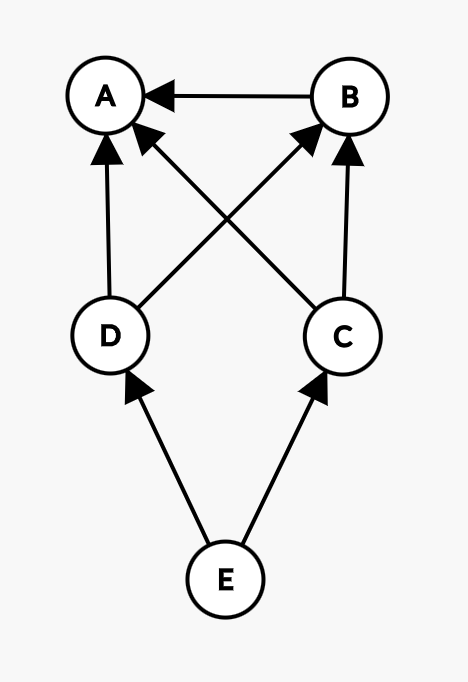
\includegraphics[height=5cm, width=3.5cm]{images/crates.png}
\end{tabular}
& \begin{tabular}{l}
    \parbox{0.6\linewidth}{
    \begin{itemize}
        \item<1-> Or the following: we've got crates \texttt{A} and \texttt{B}, in \texttt{A} there's trait, and in \texttt{B} there's a type. \texttt{B} depends on \texttt{A}. We want to use both of them as dependencies in the crate \texttt{C}. Also, there's crate \texttt{D} that depends on both \texttt{A} and \texttt{B}.
        \item<2-> Let's implement a trait from \texttt{A} for structure from \texttt{B} in \texttt{C} and \texttt{D}.
        \item<3-> In \texttt{E}, we have two implementations of trait!
    \end{itemize}
    }
\end{tabular} \\
\end{tabular}
\end{frame}

% ----------------------------------------------------------------- %

\begin{frame}[fragile]
\frametitle{Orphan rule}
To make sure the compiler will see only one implementation, there's \textit{orphan rule}.

Simply stated, the orphan rule says that you can implement a trait for a type only if the trait or the type is local to your crate (not module!).

In our example, we'll be able to implement a trait for type only in crate \texttt{B}.

In this rule, there are some exceptions.
\end{frame}

% ----------------------------------------------------------------- %

\begin{frame}[fragile]
\frametitle{Orphan rule: Blanket Implementations}
Remember: this is a \textit{blanket implementation}.

\begin{minted}{rust}
    impl<T> MyTrait for T where T: Something { /* ... */ }
\end{minted}

Only the crate that defines a trait is allowed to write a blanket implementation!

\textbf{Adding a blanket implementation to an existing trait is considered a breaking change}. If it were not, a downstream crate that contained \texttt{impl MyTrait for Foo} could suddenly stop compiling just because you update the crate that defines \texttt{MyTrait} with an error about a conflicting implementation.
\end{frame}

% ----------------------------------------------------------------- %

\begin{frame}[fragile]
\frametitle{Orphan rule: Fundamental Types}
Some types are so essential that it's necessary to allow anyone to implement traits on them.

These types currently include \texttt{\&}, \texttt{\&mut}, and \texttt{Box}. For the purposes of the orphan rule, fundamental types are erased before the orphan rule is checked.

\begin{minted}{rust}
    impl IntoIterator for &MyType { /* ... */ }
\end{minted}

With just the orphan rule, this implementation would not be permitted since it implements a foreign trait for a foreign type - \texttt{IntoIterator} and \texttt{\&} both come from the standard library.

\textbf{Note}: In standard library this types are marked by \texttt{\#[fundamental]} attribute.
\end{frame}

% ----------------------------------------------------------------- %

\begin{frame}[fragile]
\frametitle{Orphan rule: Covered Implementations}
There are some limited cases where we want to allow implementing a foreign trait for a foreign type, which the orphan rule does not normally allow:

\begin{minted}{rust}
    impl From<MyType> for Vec<i32> { /* ... */ }
\end{minted}

Here, the \texttt{From} trait is foreign, as is the \texttt{Vec} type.

Given \texttt{impl<P1..Pn> ForeignTrait<T1..Tm> for T0} is allowed only if at least one \texttt{Ti} is a local type and no \texttt{T} before the first such \texttt{Ti} is one of the generic types \texttt{P1..Pn}:

Generic type parameters (\texttt{P1..Pn}) are allowed to appear in \texttt{T0..Ti} as long as they are covered by some intermediate type. A \texttt{T} is covered if it appears as a type parameter to some other type (like \texttt{Vec<T>}), but not if it stands on its own (just \texttt{T}) or just appears behind a fundamental type like \texttt{\&T}.
\end{frame}

% ----------------------------------------------------------------- %

\begin{frame}[fragile]
\frametitle{Orphan rule: Covered Implementations}
A clarification example:

\begin{minted}[fontsize=\small]{rust}
    // 'X, Y, .., Z' - some generics
    // 'A, B, .., C' - some local types
    impl<X, Y, .., Z> ForeignTrait<u32, A, B, Vec<X>, C> for Vec<i32> {
        /* ... */
    }
\end{minted}
\end{frame}


% ----------------------------------------------------------------- %

\begin{frame}[fragile]
\frametitle{Orphan rule: Covered Implementations}
Note that:

\begin{minted}{rust}
    impl<T> ForeignTrait<LocalType, T> for ForeignType {}
\end{minted}

Is valid, but:

\begin{minted}{rust}
    impl<T> ForeignTrait<T, LocalType> for ForeignType {}
\end{minted}

Is not! Without ``generic comes after local'' rule, we could the code above, and another crate could write:

\begin{minted}{rust}
    impl<T> ForeignTrait<TheirType, T> for ForeignType {}
\end{minted}

And a conflict would arise only when the two crates were brought together. The orphan rule requires that your local type come before the type parameter.
\end{frame}

% ----------------------------------------------------------------- %

\begin{frame}[fragile,c]
\frametitle{Modules}
\begin{minted}[fontsize=\small]{rust}
    // Note the 'pub'
    pub mod one {
        pub mod nested {
            pub mod nested2 {
                pub(crate) struct Foo { bar: crate::two::Bar }
                impl crate::one::MyTrait for Foo {}
            }
            pub(self) enum Count { Example(nested2::Foo) }
        }
        trait MyTrait { /* ... */ }
    }
\end{minted}

Imagine we've put this in \texttt{lib.rs} file and published our crate. Since we added a \texttt{pub} keyword before \texttt{one}, and \texttt{one} is in our root module, everything inside became accessible for foreign crates. We don't want users to access \texttt{Foo}. One of the ways it to add \texttt{pub(crate)} visibility to \texttt{Foo}. Works just like \texttt{pub}, but only in our crate.
\end{frame}

% ----------------------------------------------------------------- %

\begin{frame}[fragile]
\frametitle{Modules}
\begin{minted}[fontsize=\small]{rust}
 pub mod one {
    pub mod nested {
        pub mod nested2 {
            pub(super) struct Foo { bar: crate::two::Bar }
            impl crate::one::MyTrait for Foo {}
        }
        pub(self) enum Count { Example(nested2::Foo) }
    }
    trait MyTrait { /* ... */ }
 }
\end{minted}

If we don't use \texttt{Foo} in any other modules than \texttt{nested2} and \texttt{nested}, there's \texttt{pub(super)} to help. It makes object available only for current module and parent module.
\end{frame}

% ----------------------------------------------------------------- %

\begin{frame}[fragile]
\frametitle{Modules}
\begin{minted}[fontsize=\small]{rust}
 pub mod one {
    pub mod nested {
        pub mod nested2 {
            pub(in crate::one::nested) struct Foo { /* ... */ }
            impl crate::one::MyTrait for Foo {}
        }
        pub(self) enum Count { Example(nested2::Foo) }
    }
    trait MyTrait { /* ... */ }
 }
\end{minted}

We can use \texttt{pub(in PATH)} to make the object visible for all ancestors from specified. For instance, in this example, we won't see \texttt{Foo} in module \texttt{one}, but all other ancestor modules will.
\end{frame}

% ----------------------------------------------------------------- %

\begin{frame}[fragile]
\frametitle{\texttt{use} keyword}
The availability of the type and definition is not the same in Rust. When you make the function public, you must have your input and output types to be at least with the same availability.

The same applies to enumerations and structures.

\begin{minted}{rust}
    mod A {
        pub mod B {
            enum Private { X }
            pub fn MyFunc(x: Private) {}
            pub enum MyEnum { Variant(Private) }
            pub struct S { pub x: Private }
        }
    }
\end{minted}
\end{frame}

% ----------------------------------------------------------------- %

\begin{frame}[fragile]
\frametitle{\texttt{use} keyword}
\begin{minted}[fontsize=\small]{rust}
error[E0446]: private type `Private` in public interface
 --> src/main.rs:4:9
  |
3 | enum Private { X }
  | ------------ `Private` declared as private
4 | pub fn MyFunc(x: Private) {}
  | ^^^^^^^^^^^^^^^^^^^^^^^^^ can't leak private type
6 | pub struct S { pub x: Private }
  | ^^^^^^^^^^^^^^ can't leak private type
\end{minted}
\end{frame}

% ----------------------------------------------------------------- %

\begin{frame}[fragile]
\frametitle{\texttt{use} keyword}
\begin{minted}[fontsize=\small]{rust}
warning: private type `Private` in public interface (error E0446)
 --> src/main.rs:5:35
  |
5 | pub enum MyEnum { Variant(Private) }
  |                           ^^^^^^^
  |
 = note: `#[warn(private_in_public)]` on by default
 = warning: this was previously accepted by the compiler
 but is being phased out; it will become a hard error in
 a future release!
 = note: for more information, see issue #34537
 <https://github.com/rust-lang/rust/issues/34537>
\end{minted}
\end{frame}

% ----------------------------------------------------------------- %

\begin{frame}[fragile,c]
\frametitle{Modules and files}
We've already seen \texttt{super} and \texttt{crate} keywords, and they was pretty close to Unix paths. It's not a coincidence! This code...

\begin{minted}[fontsize=\small]{rust}
    mod one {
        pub mod nested {
            pub mod nested2 {
                pub struct Foo { bar: crate::two::Bar }
            }
            impl crate::one::MyTrait for nested2::Foo {}
            pub(self) enum Count { Example(nested2::Foo) }
        }
        trait MyTrait { /* ... */ }
    }
    mod two {
        pub struct Bar { /* ... */ }
        pub fn use_me() { /* ... */ }
    }
\end{minted}
\end{frame}

% ----------------------------------------------------------------- %

\begin{frame}[fragile]
\frametitle{Modules and files}
...Translates to this in filesystem!

\small\begin{verbatim}
    .
    ├── Cargo.toml
    └── src
        ├── lib.rs
        ├── one
        │   ├── mod.rs
        │   └── nested
        │       ├── mod.rs
        │       └── nested2.rs
        └── two.rs
\end{verbatim}
\end{frame}

% ----------------------------------------------------------------- %

\begin{frame}[fragile]
\frametitle{Modules and files}
Well, how this works?

\begin{itemize}
    \item<1-> Every file is a module. The path to this file including it's name is module name. Exceptions - \texttt{main.rs}, \texttt{lib.rs} and \texttt{mod.rs} files. Their names ``empty'' for Rust, and everything inside them is in the root module.
    \item<2-> For instance, \texttt{two.rs} file has path \texttt{crate::two}, and \texttt{nested2.rs} - \texttt{crate::one::nested::nested2}.
\end{itemize}
\end{frame}

% ----------------------------------------------------------------- %

\begin{frame}[fragile]
\frametitle{Modules and files}
Well, how this works?

\begin{itemize}
    \item<1-> When your module contains not only code but also other modules, you should create a directory. Inside it, you'll have \texttt{mod.rs} file in which declarations will have the path of the directory.
    \item<2-> For instance, code inside \texttt{mod.rs} in \texttt{nested} have module path of \texttt{crate::one::nested}.
\end{itemize}
\end{frame}

% ----------------------------------------------------------------- %

\begin{frame}[fragile]
\frametitle{Modules and files}
Well, how this works?

\begin{itemize}
    \item<1-> Modules aren't available to the whole program by default! To include module in file, use \texttt{pub mod MODULE;} syntax: because there's no \texttt{\{\}}, Rust finds out it's not a declaration but usage of the module. File \texttt{src/one/mod.rs} contains:

    \begin{minted}{rust}
    pub mod nested;
    trait MyTrait { /* ... */ }
    \end{minted}
\end{itemize}
\end{frame}

% ----------------------------------------------------------------- %

\begin{frame}[fragile]
\frametitle{\texttt{use} keyword}
There's one convenient thing - \texttt{use} keyword.

\begin{itemize}
    \item<1-> If you want to use the name, you may want to write \texttt{use}. It's not required, but you've already seen it in homework that, for instance, writing \texttt{use std::rc::Rc} and then \texttt{Rc} is much better than writing \texttt{std::rc::Rc} everywhere.

    \begin{minted}{rust}
    use std::rc::Rc;
    let r = Rc::new(/* ... */);
    \end{minted}

    \item<2-> We can give an alias to the \texttt{use} declaration.

    \begin{minted}{rust}
    use one::nested::nested2::Foo as Test;
    let _ = Test {};
    \end{minted}
\end{itemize}
\end{frame}

% ----------------------------------------------------------------- %

\begin{frame}[fragile]
\frametitle{\texttt{use} keyword}
There's one convenient thing - \texttt{use} keyword.

\begin{itemize}
    \item<1-> The \texttt{impl} blocks for structures are available when the structure is available, and trait implementations are available when both structure and the trait are available. Moreover, to use the trait, you should first import it. When importing a trait, consider \textit{private-importing} it: it enables trait methods but won't add a name in the scope.

    \begin{minted}{rust}
    use std::io::{Write as _, BufWriter};
    \end{minted}
\end{itemize}
\end{frame}

% ----------------------------------------------------------------- %

\begin{frame}[fragile]
\frametitle{\texttt{use} keyword}
There's one convenient thing - \texttt{use} keyword.

\begin{itemize}
    \item<1-> We can import all definitions in specified module, but not nested modules, using the keyword \texttt{self}:
    
    \begin{minted}{rust}
    use std::collections::*;
    let map = HashMap::new();
    // Won't compile: hash_map is nested
    // let mut hasher = hash_map::DefaultHasher::new();
    \end{minted}
\end{itemize}
\end{frame}

% ----------------------------------------------------------------- %

\begin{frame}[fragile]
\frametitle{\texttt{use} keyword}
There's one convenient thing - \texttt{use} keyword.

\begin{itemize}
    \item<1-> Or import everything inside the module by using \texttt{*}:
    
    \begin{minted}{rust}
    mod A {
        pub mod B {
            pub enum C { X, Y }
        }
    }

    use A::*;
    let x = B::C::X;

    // Importing specific variant
    // use A::B::C::X
    // let x = X;
    \end{minted}
\end{itemize}
\end{frame}

% ----------------------------------------------------------------- %

\begin{frame}[fragile]
\frametitle{\texttt{use} keyword}
There's one convenient thing - \texttt{use} keyword.

\begin{itemize}
    \item<1-> If you want to import enum variants, you can do it by using \texttt{*}. It's how it's done in the standard library prelude with \texttt{Option} variants \texttt{Some} and \texttt{None}:
    
    \begin{minted}{rust}
    mod A {
        pub mod B {
            pub enum C { X, Y }
        }
    }

    use A::B::C*;
    let x = X;
    \end{minted}
\end{itemize}
\end{frame}

% ----------------------------------------------------------------- %

\begin{frame}
\frametitle{Questions?}
\begin{center}

\includegraphics[width=\textwidth,height=7cm,keepaspectratio]{images/crab.jpg}
\end{center}
\end{frame}

% ----------------------------------------------------------------- %

\end{document}
